% !TEX root = Dokumentation.tex
\subsection{Team}

\large
\textbf{Maschinenbau}
\begin{table}[H]
\begin{tabular}{p{0.3\textwidth}p{0.3\textwidth}}	
	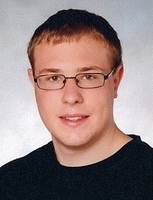
\includegraphics[width=0.25\textwidth]{./04_Projektmanagement/fig/stefanhaefliger.jpg}	&		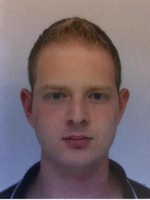
\includegraphics[width=0.25\textwidth]{./04_Projektmanagement/fig/joelmeloni.jpg} 
	\\
	\textbf{Stefan Häfliger} & 	
	\textbf{Joël Meloni}
	\\
	Beladen und Entladen &
	Chassis und Lenkung
\end{tabular}
\end{table}

\large
\textbf{Elektrotechnik}
\begin{table}[H]
\begin{tabular}{p{0.3\textwidth}p{0.3\textwidth}}	
	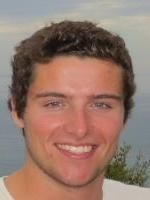
\includegraphics[width=0.25\textwidth]{./04_Projektmanagement/fig/silvanritz.jpg}	&			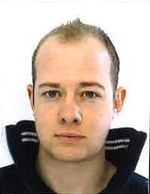
\includegraphics[width=0.27\textwidth]{./04_Projektmanagement/fig/larswalther.jpg} 
	\\
	\textbf{Silvan Ritz} & 	
	\textbf{Lars Walther}
	\\
	Servos, Sensoren und Freescale-Board &
	Energieversorgung und Antrieb
\end{tabular}
\end{table}

\newpage
\large
\textbf{Informatik}
\begin{table}[H]
\begin{tabular}{p{0.3\textwidth}p{0.3\textwidth}p{0.3\textwidth}}	
	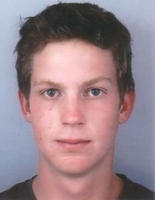
\includegraphics[width=0.26\textwidth]{./04_Projektmanagement/fig/patriziobrantschen.jpg}	&	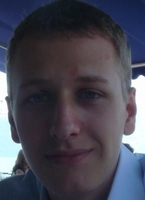
\includegraphics[width=0.24\textwidth]{./04_Projektmanagement/fig/adrianwuersch.jpg} &
	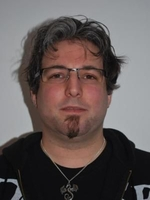
\includegraphics[width=0.25\textwidth]{./04_Projektmanagement/fig/tobiaskreienbuehl.jpg} 
	\\
	\textbf{Patrizio Brantschen} & 	
	\textbf{Adrian Würsch} &
	\textbf{Tobias Kreienbühl}
	\\
	Objekterkennung und Rechtsvortritt &
	Schnittstellen und Dokumentation &
	Fahrbahnerkennung und Mini-Computer
\end{tabular}
\end{table}
\normalsize







